\documentclass{article}
\usepackage{graphicx} % Required for inserting images
\usepackage{float}
\usepackage{listings}
\usepackage{amsmath}
\usepackage{color} % Optional, for color customization
\usepackage[margin=1in]{geometry}
\lstset{language=Matlab}



\title{MATH 543 - HW 2}
\author{Parham Khodadi}
\date{February 10, 2026}

\begin{document}

\maketitle

\section*{TB-4.1}
\subsection*{Problem}
Determine the singular value decompositions (SVDs) of the following matrices (by hand calculation):
\[
\text{(a)}\ \begin{bmatrix} 3 & 0 \\ 0 & -2 \end{bmatrix},\qquad
\text{(b)}\ \begin{bmatrix} 2 & 0 \\ 0 & 3 \end{bmatrix},\qquad
\text{(c)}\ \begin{bmatrix} 0 & 2 \\ 0 & 0 \\ 0 & 0 \end{bmatrix},\qquad
\text{(d)}\ \begin{bmatrix} 1 & 1 \\ 0 & 0 \end{bmatrix},\qquad
\text{(e)}\ \begin{bmatrix} 1 & 1 \\ 1 & 1 \end{bmatrix}.
\]


\subsection*{MATLAB code}
\begin{lstlisting}[caption={My MATLAB code for solving this question.}]
%% tb-4.1
fprintf("TB-4.1\n\n");

% Define every matrix
A_a = [3,0;0,-2];
A_b = [2,0;0,3];
A_c = [0,2;0,0;0,0];
A_d = [1,1;0,0];
A_e = [1,1;1,1];

% SVD then display U, S, V
[U_a,S_a,V_a] = svd(A_a);
fprintf("SVD of Matrix (a):\n")
fprintf("U:\n"); disp(U_a);
fprintf("S:\n"); disp(S_a);
fprintf("V:\n"); disp(V_a);
fprintf("\n");

[U_b,S_b,V_b] = svd(A_b);
fprintf("SVD of Matrix (b):\n")
fprintf("U:\n"); disp(U_b);
fprintf("S:\n"); disp(S_b);
fprintf("V:\n"); disp(V_b);
fprintf("\n");

[U_c,S_c,V_c] = svd(A_c);
fprintf("SVD of Matrix (c):\n")
fprintf("U:\n"); disp(U_c);
fprintf("S:\n"); disp(S_c);
fprintf("V:\n"); disp(V_c);
fprintf("\n");

[U_d,S_d,V_d] = svd(A_d);
fprintf("SVD of Matrix (d):\n")
fprintf("U:\n"); disp(U_d);
fprintf("S:\n"); disp(S_d);
fprintf("V:\n"); disp(V_d);
fprintf("\n");

[U_e,S_e,V_e] = svd(A_e);
fprintf("SVD of Matrix (e):\n")
fprintf("U:\n"); disp(U_e);
fprintf("S:\n"); disp(S_e);
fprintf("V:\n"); disp(V_e);
fprintf("\n");

fprintf("-----------------\n");
\end{lstlisting}

\subsection*{Output}
\begin{verbatim}
TB-4.1

SVD of Matrix (a):
U:
     1     0
     0     1

S:
     3     0
     0     2

V:
     1     0
     0    -1


SVD of Matrix (b):
U:
     0     1
     1     0

S:
     3     0
     0     2

V:
     0     1
     1     0


SVD of Matrix (c):
U:
     1     0     0
     0     1     0
     0     0     1

S:
     2     0
     0     0
     0     0

V:
     0    -1
     1     0


SVD of Matrix (d):
U:
    1.0000         0
         0    1.0000

S:
    1.4142         0
         0         0

V:
    0.7071   -0.7071
    0.7071    0.7071


SVD of Matrix (e):
U:
   -0.7071   -0.7071
   -0.7071    0.7071

S:
    2.0000         0
         0    0.0000

V:
   -0.7071    0.7071
   -0.7071   -0.7071


-----------------
\end{verbatim}

\newpage
\section*{TB-4.3}
\subsection*{Problem}
Write a MATLAB program (see Lecture 9) which, given a real $2\times2$ matrix $A$, plots the right singular vectors $v_1$ and $v_2$ in the unit circle and also the left singular vectors $u_1$ and $u_2$ in the appropriate ellipse, as in Figure 4.1. Apply your program to the matrix (3.7) and also to the $2\times2$ matrices of Exercise 4.1.

\subsection*{MATLAB code}
\begin{lstlisting}[caption={My MATLAB code for solving this question.}]
%% tb-4.3
fprintf("TB-4.3\n\n");

% Ask for Matrix
A = zeros(2,2);
fprintf("Please input the value for each element in the 2x2 matrix A, below\n");
A(1,1) = input("A_11 = ");
A(1,2) = input("A_12 = ");
A(2,1) = input("A_21 = ");
A(2,2) = input("A_22 = ");

% SVD
[U,S,V] = svd(A);
sigma1 = S(1,1);
sigma2 = S(2,2);
v1 = V(:,1);
v2 = V(:,2);
u1 = U(:,1);
u2 = U(:,2);

% Display SVD
fprintf("Singular values of matrix A:\n");
fprintf("Sigma1 = %.4f\nSigma2 = %.4f\n", sigma1, sigma2);
fprintf("v1 = [%.6g; %.6g], v2 = [%.6g; %.6g]\n", v1(1), v1(2), v2(1), v2(2));
fprintf("u1 = [%.6g; %.6g], u2 = [%.6g; %.6g]\n\n", u1(1), u1(2), u2(1), u2(2));

% Unit Circle + V
t = linspace(0, 2*pi, 31415);
X = [cos(t); sin(t)];
Y = A*X;

figure;
plot(X(1,:), X(2,:), 'k', 'LineWidth', 1.5); hold on; grid on;
quiver(0,0, v1(1), v1(2), 0, 'LineWidth', 2, 'MaxHeadSize', 0.25);
quiver(0,0, v2(1), v2(2), 0, 'LineWidth', 2, 'MaxHeadSize', 0.25);
axis equal;
xlabel('x'); ylabel('y');
title('Unit circle with right singular vectors');
legend('unit circle','$v_1$','$v_2$','Location','best','Interpreter','latex');
exportgraphics(gcf, 'unit_circle_V.eps', 'ContentType', 'vector');


% Ellipse + Sigma*U
p1 = sigma1*u1;
p2 = sigma2*u2;

figure;
plot(Y(1,:), Y(2,:), 'k', 'LineWidth', 1.5); hold on; grid on;
quiver(0,0, p1(1), p1(2), 0, 'LineWidth', 2, 'MaxHeadSize', 0.25);
quiver(0,0, p2(1), p2(2), 0, 'LineWidth', 2, 'MaxHeadSize', 0.25);
axis equal;
xlabel('x'); ylabel('y');
title('Ellipse with left singular vectors');
legend('ellipse','$\sigma_1 u_1$','$\sigma_2 u_2$','Location','best',
'Interpreter','latex');
exportgraphics(gcf, 'ellipse_U.eps', 'ContentType', 'vector');
\end{lstlisting}

\subsection*{Output}
\subsubsection{When using matrix (3.7)}
Matrix (3.7) in the book is $A =\begin{bmatrix} 1 & 2 \\ 0 & 2 \end{bmatrix}$.

Here's the console output from this code:

\begin{verbatim}
TB-4.3
    
Please input the value for each element in the 2x2 matrix A, below
A_11 = 1
A_12 = 2
A_21 = 0
A_22 = 2
Singular values of matrix A:
Sigma1 = 2.9208
Sigma2 = 0.6847
v1 = [0.256668; 0.9665], v2 = [-0.9665; 0.256668]
u1 = [0.749678; 0.661803], u2 = [-0.661803; 0.749678]
\end{verbatim}

The following figures (Figures \ref{fig:1_unit_circle_V} and \ref{fig:1_ellipse_U}) are generated.

\begin{figure}[H]
    \centering
    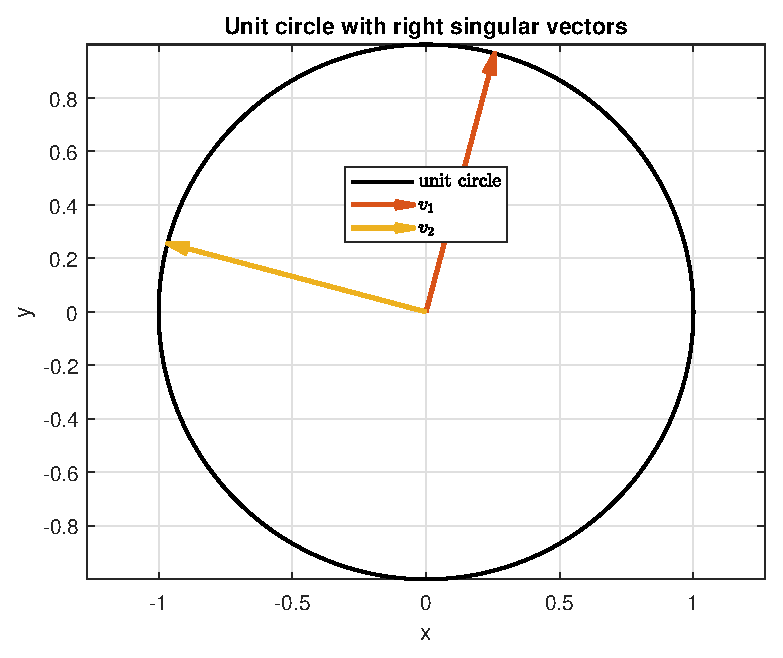
\includegraphics[width=0.7\linewidth]{Figures/1_unit_circle_V.eps}
    \caption{Unit circle with right singular vectors $v_1$ and $v_2$.}
    \label{fig:1_unit_circle_V}
\end{figure}

\begin{figure}[H]
    \centering
    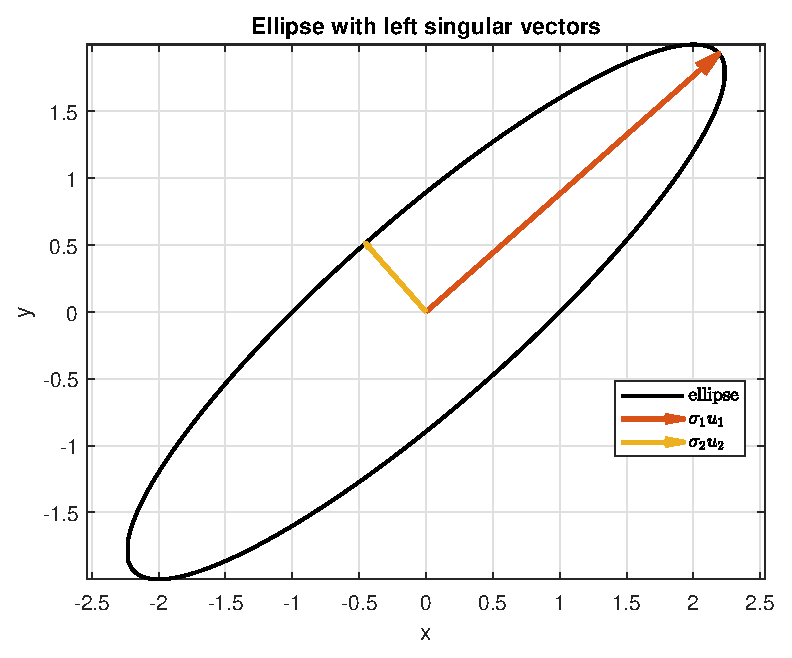
\includegraphics[width=0.7\linewidth]{Figures/1_ellipse_U.eps}
    \caption{Ellipse with singular values times left singular vectors $\sigma_1u_1$ and $\sigma_2 u_2$.}
    \label{fig:1_ellipse_U}
\end{figure}

\subsubsection{The $2\times2$ Matrices in Problem 4.1}
\subsubsection*{(a)}
\begin{figure}[H]
    \centering
    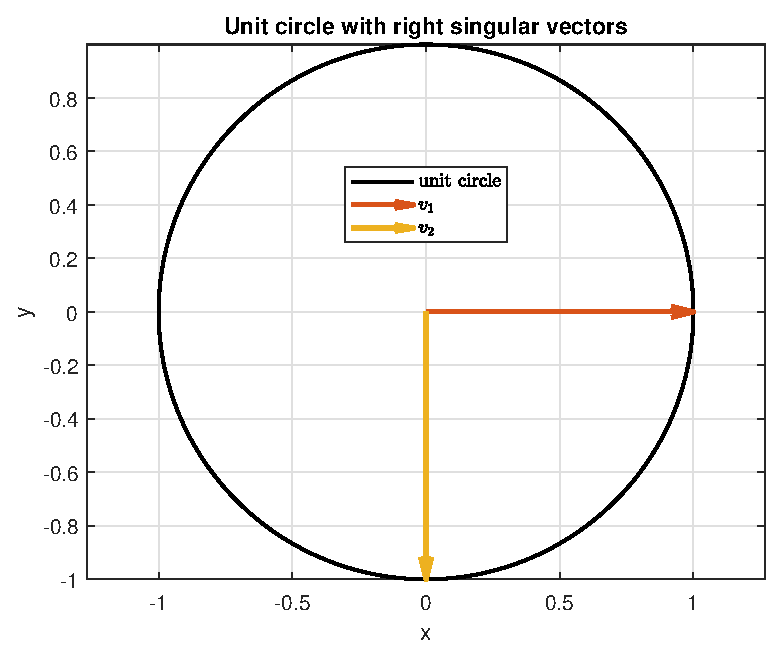
\includegraphics[width=0.7\linewidth]{Figures/a_unit_circle_V.eps}
    \label{fig:a_unit_circle_V}
\end{figure}

\begin{figure}[H]
    \centering
    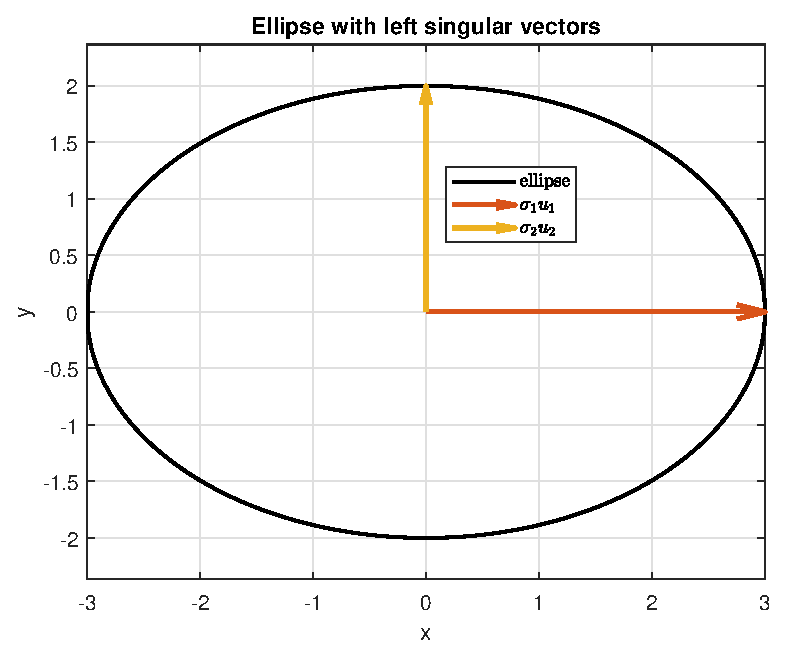
\includegraphics[width=0.7\linewidth]{Figures/a_ellipse_U.eps}
    \label{fig:a_ellipse_U}
\end{figure}

\subsubsection*{(b)}
\begin{figure}[H]
    \centering
    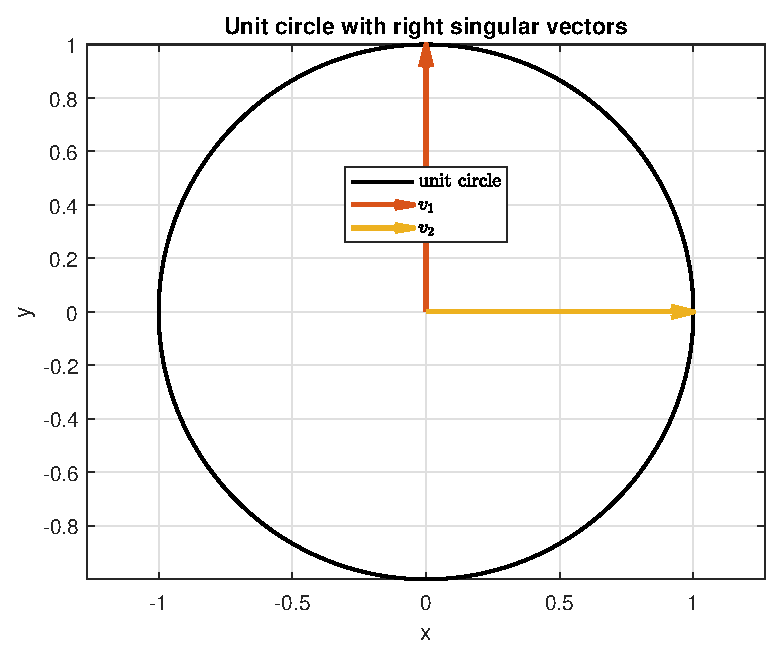
\includegraphics[width=0.7\linewidth]{Figures/b_unit_circle_V.eps}
    \label{fig:b_unit_circle_V}
\end{figure}

\begin{figure}[H]
    \centering
    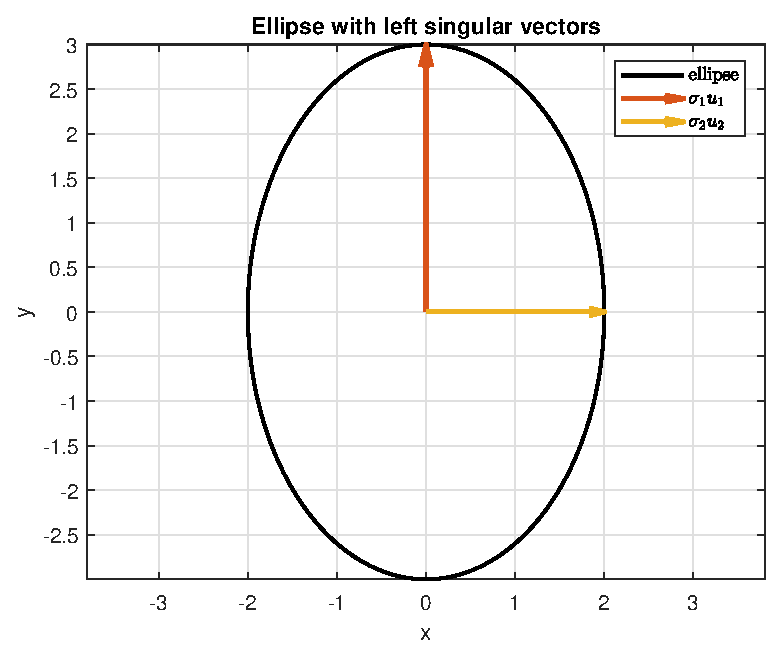
\includegraphics[width=0.7\linewidth]{Figures/b_ellipse_U.eps}
    \label{fig:b_ellipse_U}
\end{figure}


\subsubsection*{(d)}
\begin{figure}[H]
    \centering
    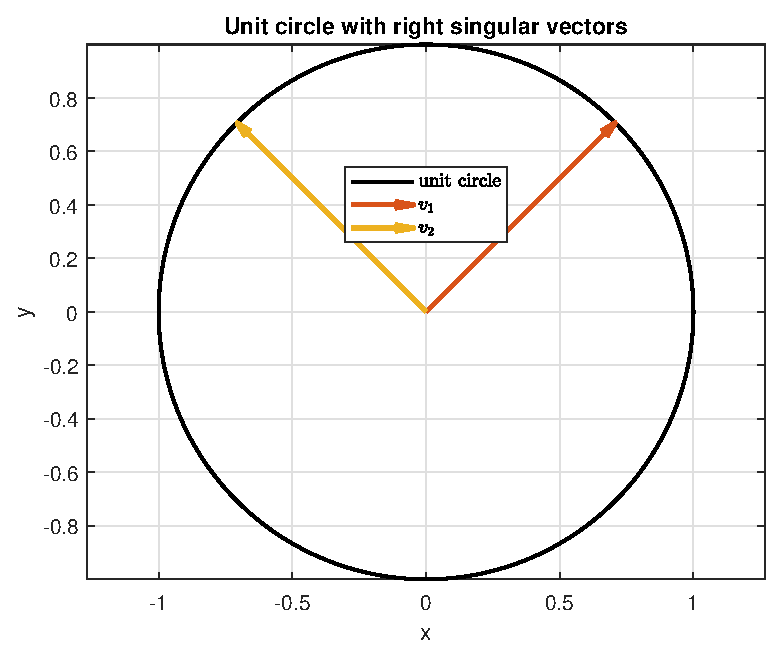
\includegraphics[width=0.7\linewidth]{Figures/d_unit_circle_V.eps}
    \label{fig:d_unit_circle_V}
\end{figure}

\begin{figure}[H]
    \centering
    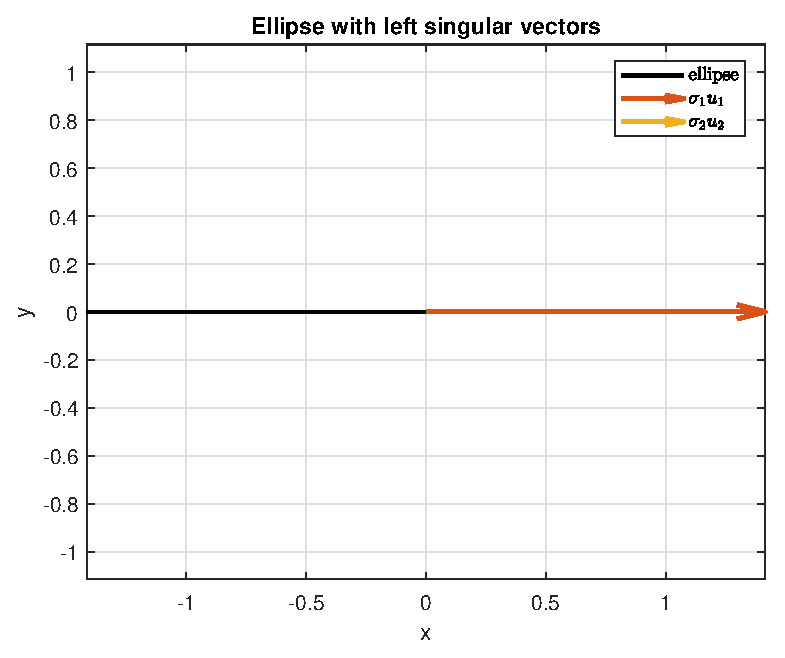
\includegraphics[width=0.7\linewidth]{Figures/d_ellipse_U.eps}
    \label{fig:d_ellipse_U}
\end{figure}

\subsubsection*{(e)}
\begin{figure}[H]
    \centering
    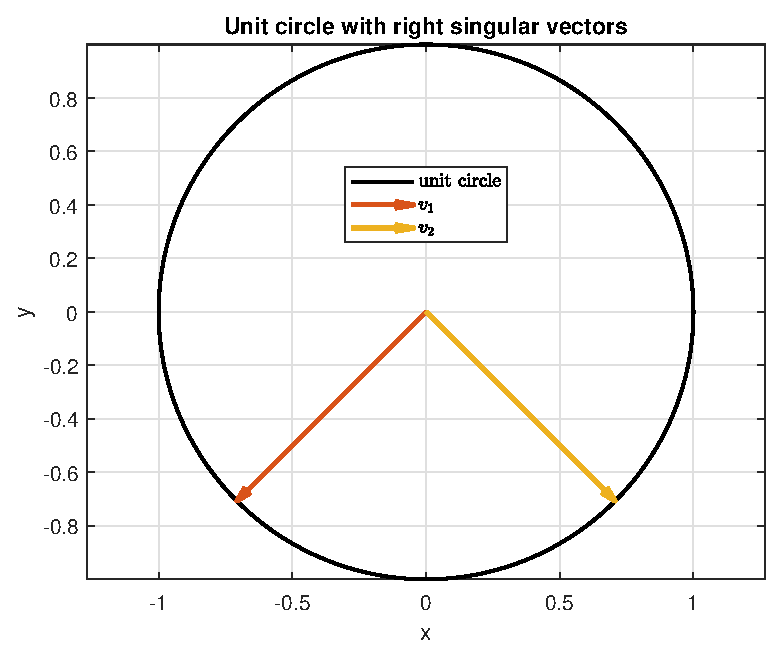
\includegraphics[width=0.7\linewidth]{Figures/e_unit_circle_V.eps}
    \label{fig:e_unit_circle_V}
\end{figure}

\begin{figure}[H]
    \centering
    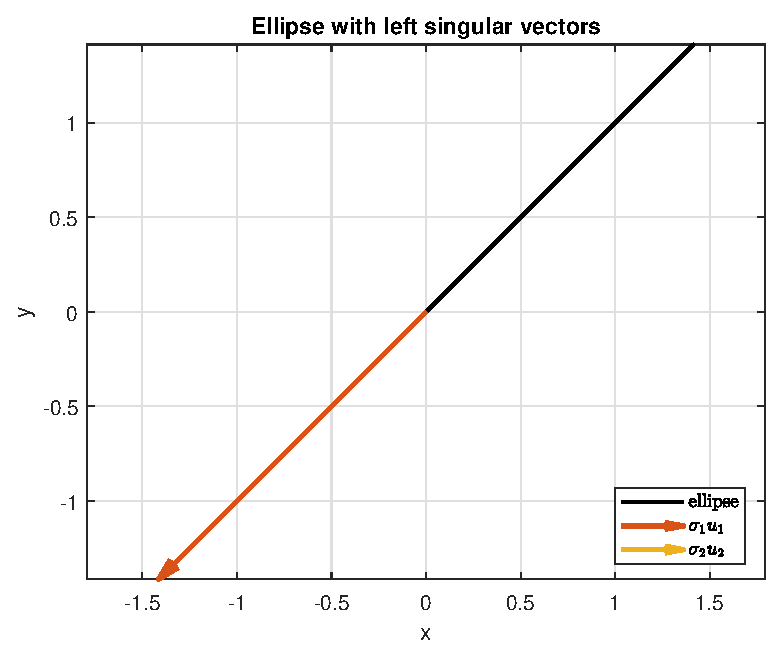
\includegraphics[width=0.7\linewidth]{Figures/e_ellipse_U.eps}
    \label{fig:e_ellipse_U}
\end{figure}


\end{document}
